% ##################################################################################################################
\chapter{Rotterdam: Revenue Management in Public Transportation with Smart-Card Data Enabled Agent-Based Simulations \textsuperscript{\footnotesize{\footnote{This research was conducted at Rotterdam School of Management and
supported by Netherlands Organisation for Scientific Research (NWO)
Complexity Grant No. 645.000.001 awarded to Dr. Ting Li and Prof.mr.dr. Peter Vervest from
Rotterdam School of Management. It was presented at \protect\gls{matsim} User Meetings in 2011 and 2012,
INFORMS International 2012 Beijing, the 7th Workshop on Agents in Traffic and Transportation at
AAMAS 2012 Valencia, Erasmus University Rotterdam, Berlin Institute of Technology, Tsinghua
University and Beijing Jiaotong University.}}}}
\label{ch:rotterdam}
\hfill \textbf{Authors:} Paul Bouman, Milan Lovric

\editdone{This text has undergone the professional edit. Please no grammatical changes anymore! They are most-probably wrong.}

% ##################################################################################################################
In \citet[][]{LovricEtAl_DSS_2013} and \citet[][]{BoumanEtAl_AAMAS_2012}, we proposed two scenarios for studying public transportation revenue management via time-based pricing strategies, like peak markups and off-peak discounts, currently being used by various transit agencies. To evaluate this approach, we developed agent-based simulations using \gls{matsim} and a transportation demand generated from smart-card data collected in a Dutch urban area. In the first scenario, we simulated only a metro network, while in the second scenario we considered a \gls{multimodal} network, consisting of metro, tram and bus.

In \citet[][]{LovricEtAl_DSS_2013}, we designed and implemented a decision support system for sustainable revenue management to evaluate the impact of various revenue management strategies on economic, social, and environmental performance. Figure~\ref{fig:rotterdam} shows the decision support system structure built on top of the \gls{matsim} framework. Smart card transactions (individual check-in and check-out transactions made at stations' entrance and exit gates) were used to reconstruct individual passenger's daily tours. These were inputted into \gls{matsim} as initial demand; information about the transit network and vehicle schedule was extracted from the \gls{osm} data and the public transit operator's web site, respectively. Revenue management experiments were then conducted by applying various time-based pricing strategies defined as percentage-wise discounts or markups (applied on top of the nominal price) during specific periods of the day. 

\gls{matsim}'s loop (Section~\ref{sec:inbrief}) was adapted for studying time-based pricing. First, an event handler was created to calculate whole daily tour travel fare for each individual (this was implemented using the real-life pricing scheme: a fixed fee applied at check-in, plus a variable distance-based fee applied at check-out). Second, we adapted the original Charypar-Nagel scoring function \citep[][]{CharyparNagel2005ga4acts}, by adding travel fare disutility. The existing \gls{matsim}'s time mutator was used as a replanning strategy, allowing passengers to discover more affordable travel times when pricing strategies were enforced (however, a trade-off was introduced by applying a penalty for arriving outside the expected arrival window, based on the observed smart card data check-out times).

To capture revenue management impact on the three sustainability dimensions, we added event handlers to produce a number of relevant \glspl{kpi}. The economic performance was measured by \gls{pto}, passenger kilometers revenue and vehicle load factors. Social performance was measured by seat availability (a proxy for passenger comfort), calculated from vehicle loadings after the mobility simulation. We also looked at average tour price as the measure of public transportation affordability. Impact of a pricing policy on the environment was expressed as the change in carbon footprint occurring through a demand shift between public transportation and private cars (calculated from average tour price change and demand elasticity). 

Our results showed that, by using a smart-card enabled decision support system and taking a customer-centric view, \glspl{pto} can better explore feasible solutions in a broader policy-making context that includes three dimensions of people-profit-planet sustainability. We validated our approach by comparing the simulation-generated travel fares in the nominal scenario with actual fares recorded in the smart card transactional database \citep[see][]{LovricEtAl_DSS_2013}.

To further study smart card data opportunities in demand generation, \citet[][]{BoumanEtAl_AAMAS_2012}, we introduced a pattern-based demand generation method using three different modalities' (metro, tram and bus) smart card transactions in a Netherlands urban area as input. In addition to using single day observations to generate activity-based demand, daily commuting patterns detected from longitudinal observations for a single smart card were generated. In this study, generated demands were utilized to analyze time-shifting behavior under two different revenue management policies: a plain tariff (with a fixed price per journey and a price per unit of traveled distance) and an off-peak discount. The experiment was repeated for different levels of pattern-based demand, where the varied parameter was the number of observed samples required for a smart card to be included. 

In generated demand, agents not generated using pattern-based demand had to replicate their observed tour or trip within 15\,minute windows of observed arrival and departure times. Pattern-based agents had time windows dependent on observed standard deviations in passengers' actual commuting travel patterns, which were used as a proxy for their time flexibility. This aspect of demand modeling was more detailed than \citet[][]{LovricEtAl_DSS_2013}, where agents were assumed to be homogeneous about their time flexibility. This flexibility was exploited by the time shift mutator, made available in \gls{matsim} as one of the \gls{replanning} strategies. In future work, improvements in scoring function and use of more sophisticated pattern-based demand generation approach must be considered to create more realistic scenarios for a study of time-shifting behavior under revenue management policies.

\createfigure%
{Rotterdam scenario}%
{Rotterdam scenario: Decision support system for sustainable revenue management in public transportation}%
{\label{fig:rotterdam}}%
{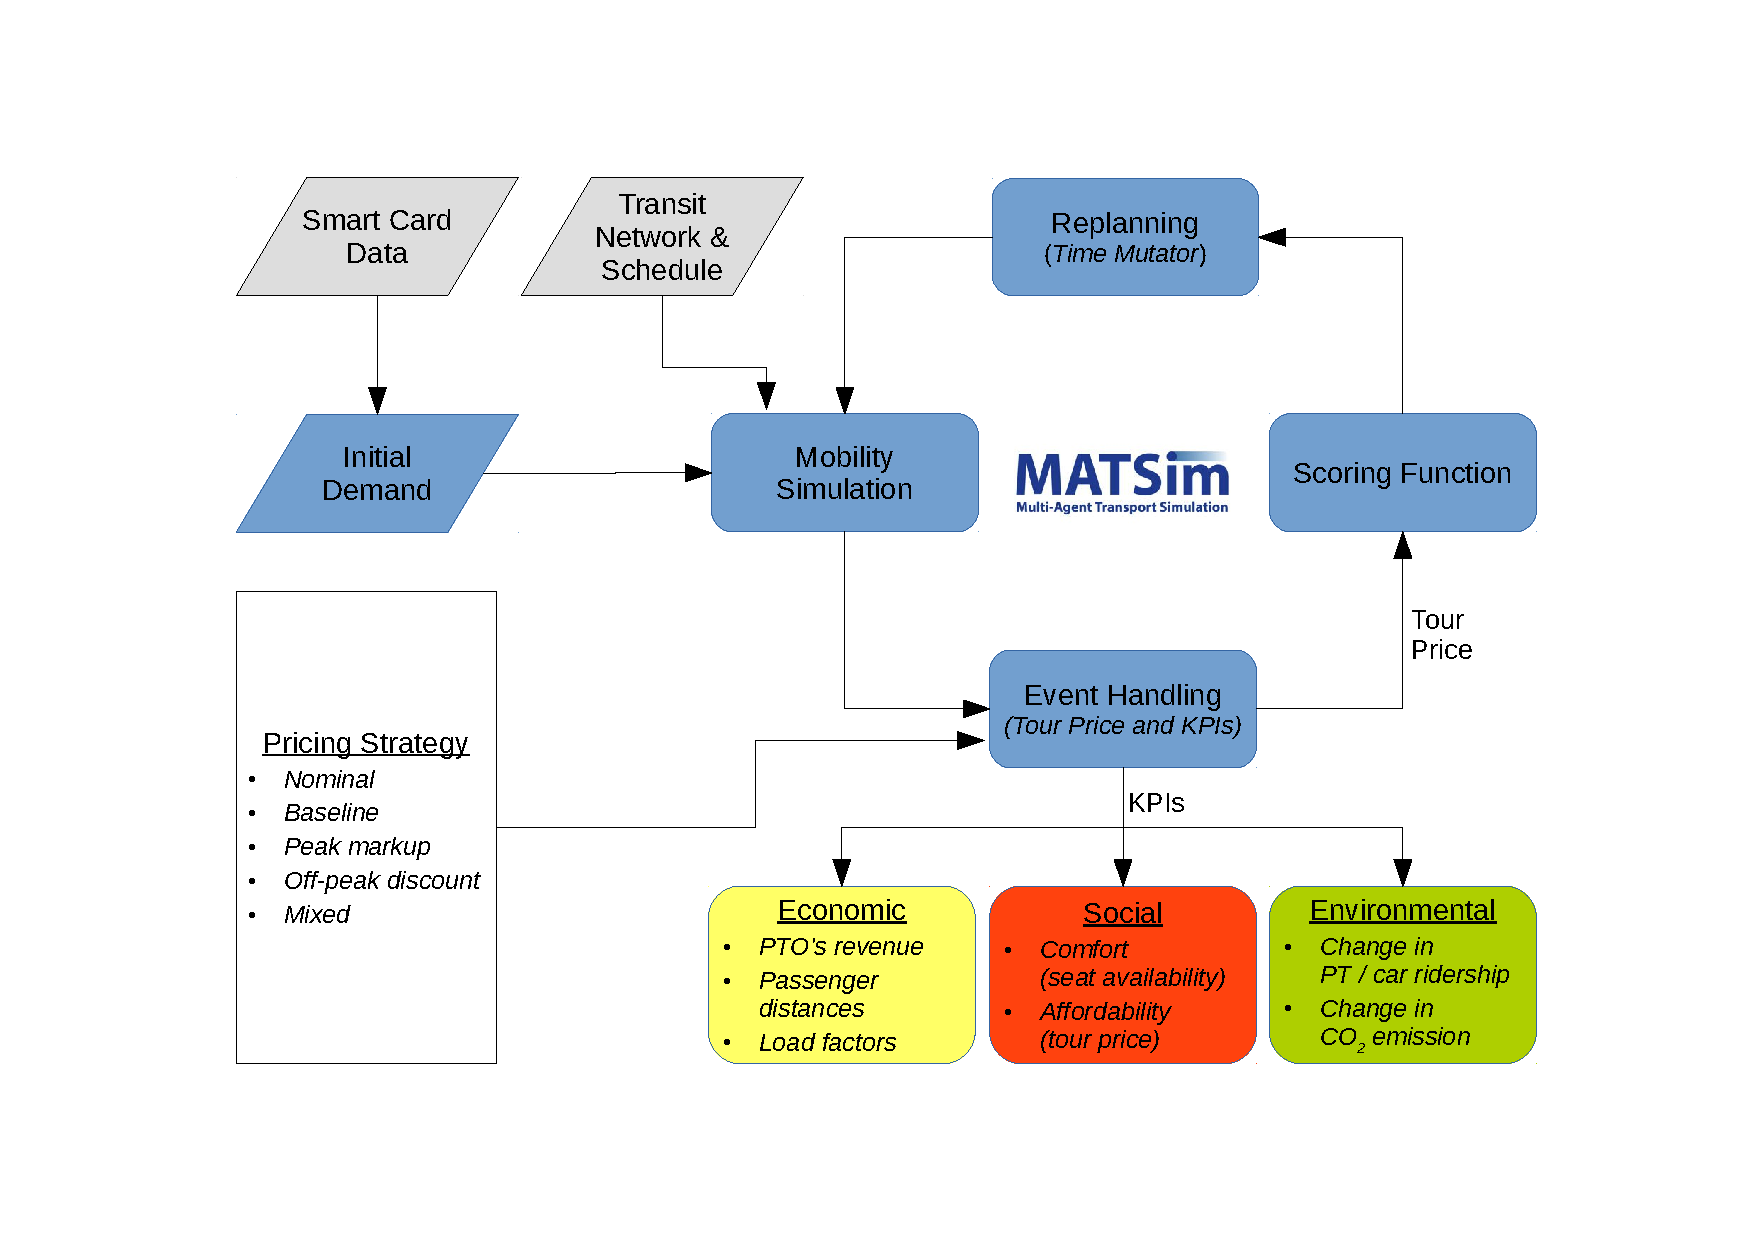
\includegraphics[width=0.85\textwidth, angle=0]{./scenarios/figures/rotterdam}}%
{}

% ##################################################################################################################

